\section{Introduction and Fundamentals}
\frame{\tableofcontents[currentsection]}
	\subsection{Introduction}
	\begin{frame}
		\frametitle{Introduction}
		kurzes blabla
	\end{frame}
	\begin{frame}
		\frametitle{Flow Properties}
		compressible flow \\
		ideal gas mit gamma
		Ma = def , 0.2
		Re, Pr	
	\end{frame}
	\begin{frame}
		\frametitle{Compressible Navier-Stokes Equation}
		2d\\
		conserved flow variables density, momentum, energy\\
		dimensionless variables\\
		gleichung, aufgeteilt in temporal derivative, convective fluxes, viscous fluxes\\
		time discretisation durch Runge-Kutta erster Ordnung -> expliziter Euler
	\end{frame}
	\subsection{The Discontinuous Galerkin Method}
	\begin{frame}
		\frametitle{The Discontinuous Galerkin Space Discretisation}
		\begin{figure}
			\centering
			\subfloat[First order FEM \label{fig:a}]{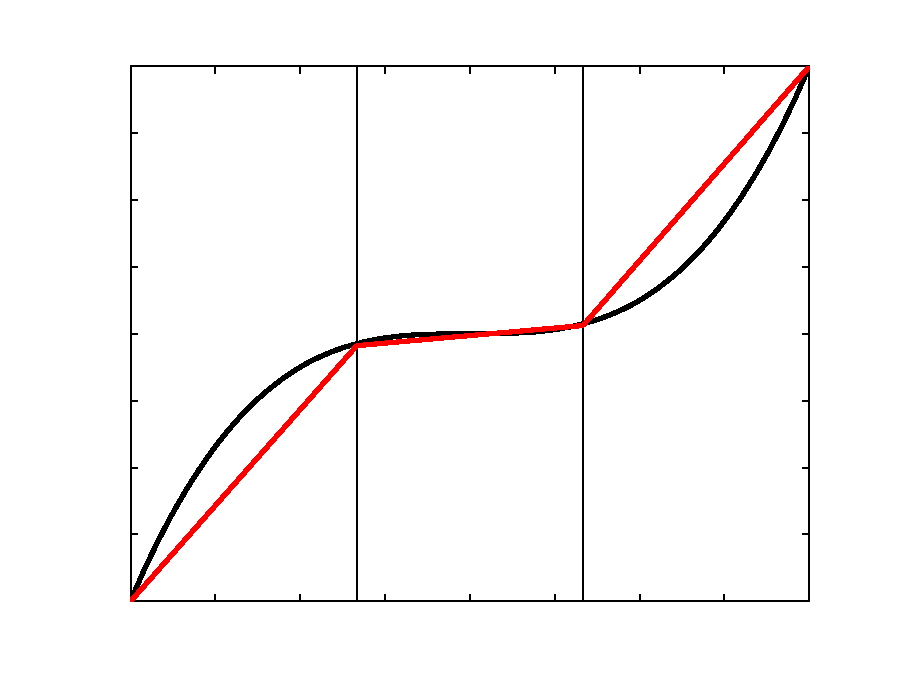
\includegraphics[width=0.28\textwidth]{img/fem.eps}}
			\subfloat[Zeroth order DG (FVM)\label{fig:b}]{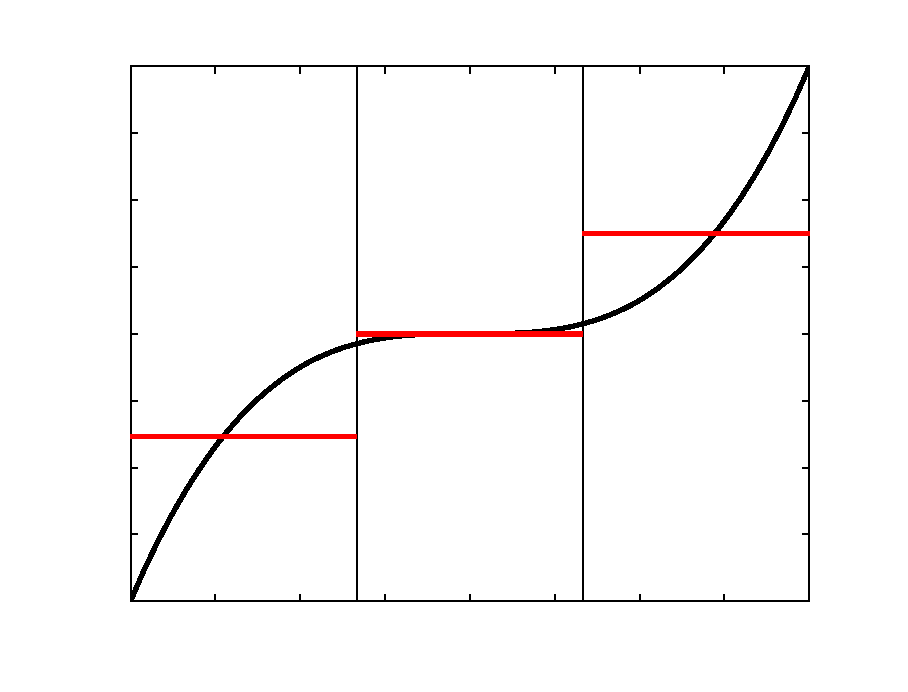
\includegraphics[width=0.28\textwidth]{img/fvm.eps}}
			\subfloat[First order DG \label{fig:c}]{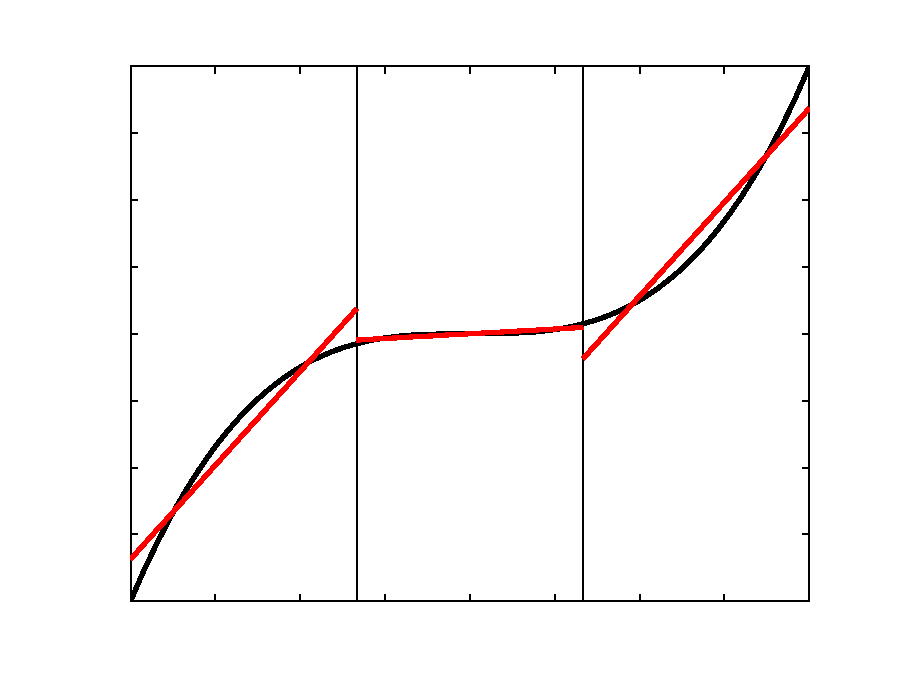
\includegraphics[width=0.28\textwidth]{img/dg.eps}}
			\caption{Comparison of FEM, FVM and DG}
			\label{fig:1}
		\end{figure}

		DG space discretisation Vorgehen, Bildchen, fluxes
	\end{frame}
	\subsection{The Immersed Boundary Method}
	\begin{frame}
		\frametitle{The Immersed Boundary Method}
		\begin{columns}[t]
			\column[]{7cm}
			\column[]{5cm}
			\begin{figure}[htbp]
				\vspace{-1cm}
				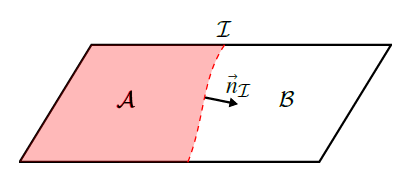
\includegraphics[width=\textwidth]{img/ibmcut.PNG}
				\caption{Cut cell with physical (red) and void region (white) [4]}\label{fig:cutcell}
			\end{figure} 
		\end{columns}
		regions mit Bild, Aufteilung Integrale
		mass matrix
		rk time discretisation formel
		cell agglomeration
	\end{frame}
	\begin{frame}
		\frametitle{Cell Agglomeration}
		\begin{columns}[t]
			\column[]{7cm}
			\column[]{5cm}
			\begin{figure}[htbp]
				\vspace{-1cm}
				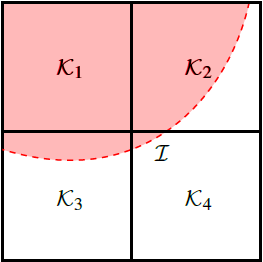
\includegraphics[height=0.3\textheight]{img/ibminitmesh.PNG}
				\caption*{(a) Initial mesh partitioning}
				\label{fig:init}
			\end{figure} 
			\begin{figure}[htbp]
				\vspace{-1cm}
				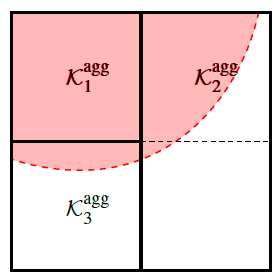
\includegraphics[height=0.3\textheight]{img/ibmagglomklein.PNG}
				\caption*{(b) Cell agglomeration with small agglomeration threshold}
				\label{fig:ineit}
			\end{figure} 
			\begin{figure}[htbp]
				\vspace{-1cm}
				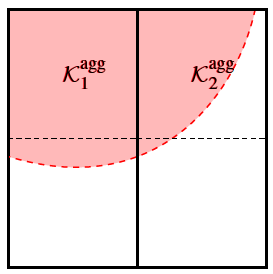
\includegraphics[height=0.3\textheight]{img/ibmagglomgross.PNG}
				\caption*{(c) Cell agglomeration with bigger agglomeration threshold}
				\label{fig:iwnit}
			\end{figure} 
		\end{columns}
		regions mit Bild, Aufteilung Integrale
		mass matrix
		rk time discretisation formel
		cell agglomeration
	\end{frame}